\chapter{Technologies}

Below the technologies and libraries used to develop the system:

\begin{itemize}
    \item \textbf{Protelis} $\rightarrow$ for the aggregate program
    \item \textbf{DingNet simulator} \footnote{\href{https://github.com/dimoibiehg/DingNet}{DingNet}} $\rightarrow$ as simulator for LoRaWan network. DingNet simulator was chosen for two reason: it provide also a real network where is possible deploy the simulated application, and there is the possibility to modify it if needed.  
    \item \textbf{MQTT} $\rightarrow$ for the communication between:
    \begin{itemize}
        \item LoRaWan network and Protelis backend
        \item Protelis nodes to exchange neighborhood information
        \item Protelis nodes and Neighborhood-Manager
    \end{itemize}
    \item \textbf{Kotlin} $\rightarrow$ to implement the Protelis backend
    \item \textbf{Java v.11} $\rightarrow$ to work on the DingNet simulator that is in Java
    \item \textbf{Eclipse Paho MQTT client library}\footnote{\href{https://github.com/eclipse/paho.mqtt.java}{MQTT library}} $\rightarrow$ to implement a MQTT client for a real MQTT broker
\end{itemize}

\section{DingNet simulator}
DingNet is a simulator for a LoRaWan network of class A. It allows to:
\begin{itemize}
    \item define different types of devices
    \item configure the network parameter for each device and gateway
    \item simulate the communication between devices and gateways in both the directions
    \item configure the position in the environment of devices and gateways
    \item add different kind of sensors to each device 
    \item define the path that a device has to follow
\end{itemize}
DingNet provide a LoRa-over-Mqtt architecture, \autoref{fig:dingARch}, so all the communications from gateways to network server to applications and the opposite are based on MQTT. The network server publishes messages for application on the topic \mintinline{java}{"application/applicationID/node/nodeID/rx"}, the message contains the packet sent from the device and all the information available on the transmission. To send a message from the application to one device, the application has to publishes it on the topic \mbox{\mintinline{java}{"application/applicationID/node/nodeID/tx"}} and the message has to contain the payload of the message and the list of mac command.

\begin{figure}[h]
    \centering
    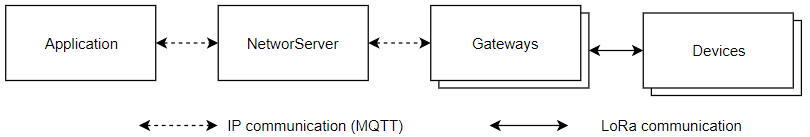
\includegraphics[scale=0.8]{images/dingNet-arch.png}
    \caption{High-level architecture of DingNet simulator. All the communications between gateways and devices use LoRa technology. While the other communications are Internet-based, and in this case use MQTT. This difference is also visible from the different kind of arrows used.}
    \label{fig:dingARch}
\end{figure}
\clearpage
How it works:
\begin{itemize}
    \item the simulator is single threaded
    \item the simulator is "time-based" with a global clock that schedules all the computations
    \item every device sends a packet every X seconds. If the packet is the same as the previous one, the packet isn't sent to avoid use of bandwidth for useless message
    \item if a device doesn't send any message for Y seconds (with Y $>$ X) then the device sends a message to confirm the previous one
    \item when a gateway receives a message from a device, it publishes the message on MQTT
    \item a gateway can use different strategies to send a message to a device: send it only after receive a message from that device, send it immediately after received it, ...
    \item a device can receive only one message after every sent message
    \item during a simulation step:
    \begin{itemize}
        \item every device consumes its packet, if it has one
        \item every movable device moves of one meter if it is pass enough time according to the movement speed
        \item at the end the global clock is increment of one tick (now 1 millisecond)
    \end{itemize}
    \item when the global clock is incremented, it checks if are present some event to fire. Now the events present are: 
    \begin{itemize}
        \item send packet every X and Y seconds
        \item packet arrived to destination
        \item define transmitting window sender side, to avoid to send more message at the same time or receiving a message during a transmission
    \end{itemize}
\end{itemize}